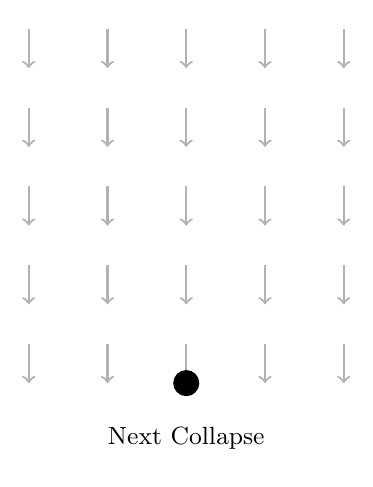
\begin{tikzpicture}[
    vec/.style={->, thick, draw=gray!60},
]

\foreach \x in {-2,-1,0,1,2}{
    \foreach \y in {-2,-1,0,1,2}{
        \draw[vec] (\x,\y) -- ++(0,-0.5);
    }
}

\node[circle, fill=black, minimum size=6pt] at (0,-2.5) {};
\node at (0,-3.2) {\small Next Collapse};

\end{tikzpicture}